\documentclass[tikz,border=6pt]{standalone}
\usepackage{tikz}
\begin{document}
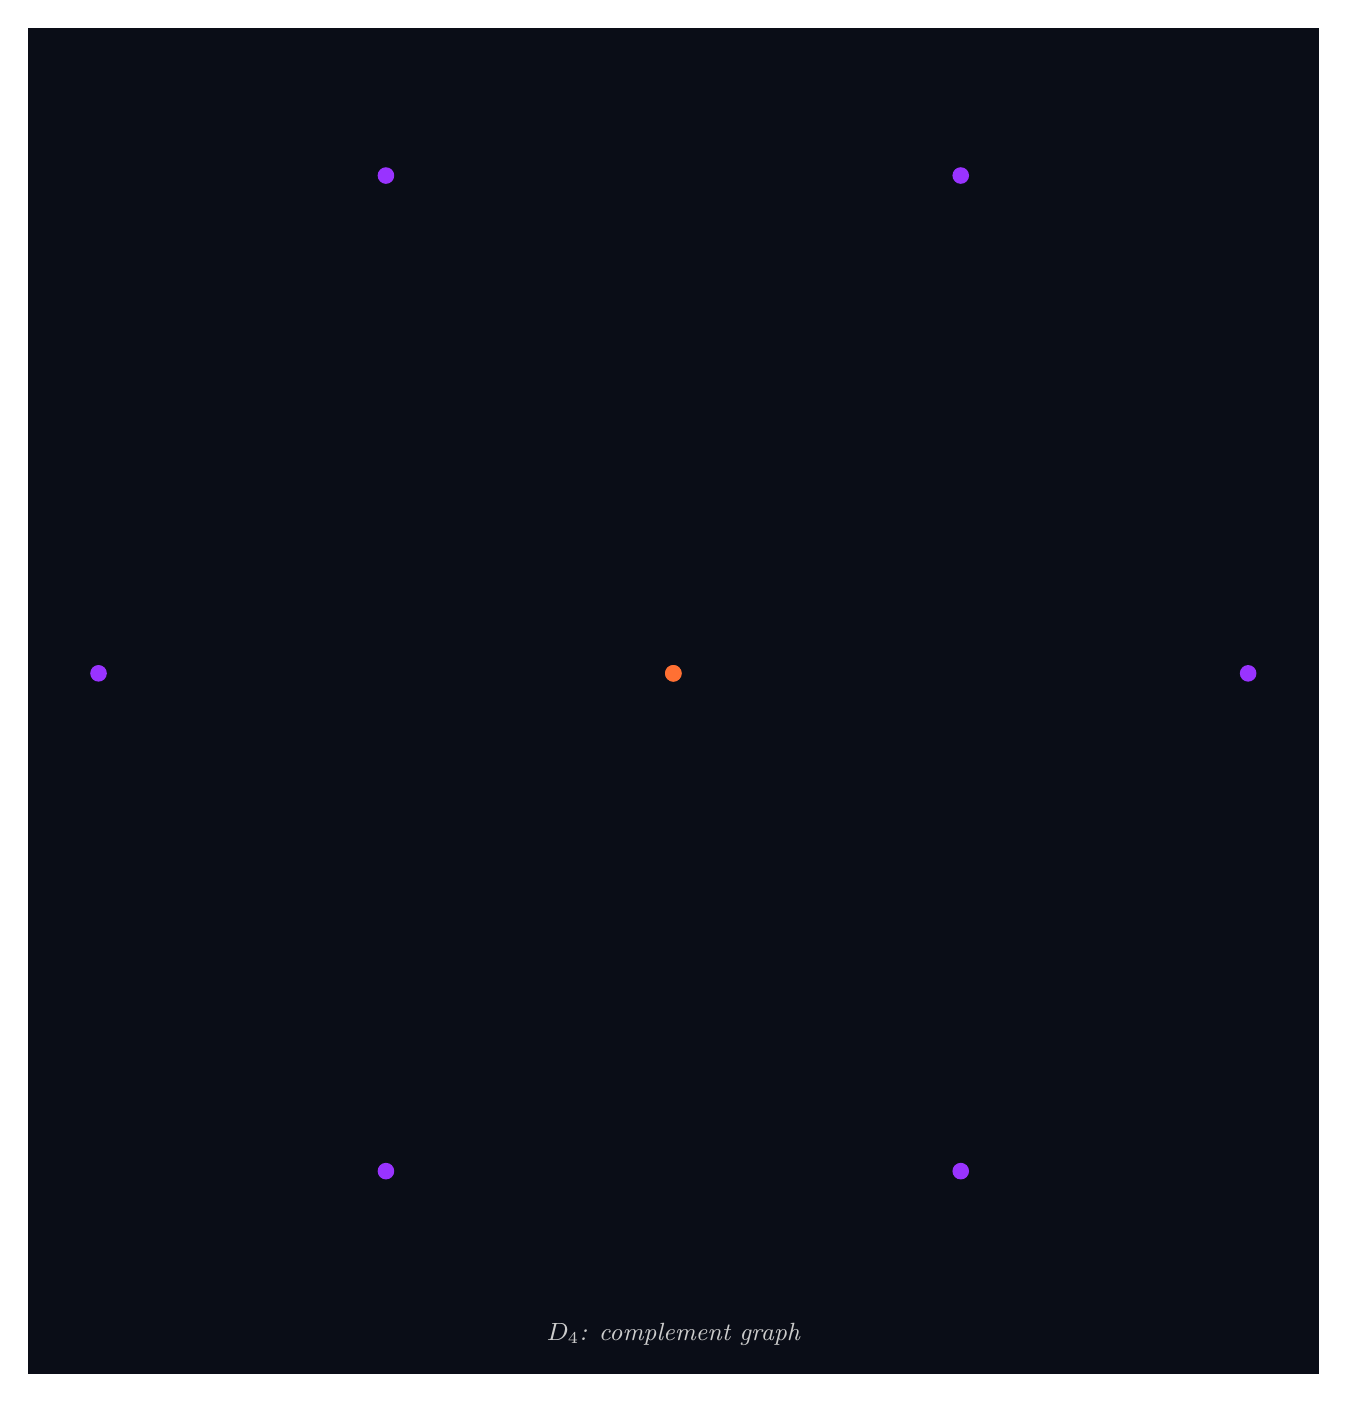
\begin{tikzpicture}
\definecolor{ring0}{rgb}{1.000,0.440,0.200}
\definecolor{ring1}{rgb}{0.600,0.200,1.000}
\definecolor{bg}{rgb}{0.04,0.05,0.09}
\fill[bg] (-8.2,-8.9) rectangle (8.2,8.2);
\fill[ring1] (-3.650,-6.322) circle (3.0pt);
\fill[ring1] (7.300,-0.000) circle (3.0pt);
\fill[ring0] (0.000,0.000) circle (3.0pt);
\fill[ring1] (-3.650,6.322) circle (3.0pt);
\fill[ring1] (3.650,-6.322) circle (3.0pt);
\fill[ring0] (-0.000,-0.000) circle (3.0pt);
\fill[ring1] (-7.300,0.000) circle (3.0pt);
\fill[ring1] (3.650,6.322) circle (3.0pt);
\node[white!80!black,font=\small\itshape] at (0,-8.4) {$D_4$: complement graph};
\end{tikzpicture}
\end{document}